\documentclass[a4paper,fleqn]{cas-dc}

\usepackage[authoryear]{natbib}
\usepackage{amsmath}
\usepackage{amsfonts}
\usepackage{amssymb}
\usepackage{booktabs}
\usepackage{tikz}
\usetikzlibrary{shapes.geometric, arrows.meta, positioning, fit, backgrounds}

\begin{document}
\let\WriteBookmarks\relax
\def\floatpagepagefraction{1}
\def\textpagefraction{.001}

\shorttitle{Hierarchical Deep Learning for Carbonate Microfacies}
\shortauthors{Authors et~al.}

\title[mode=title]{Deep learning-based classification of carbonate microfacies components in thin-section images}

\author[1]{Musawer Muradi}[orcid=0000-0001-0000-0000]
\cormark[1]
\ead{musavir.muradi@gmail.com}
\credit{Conceptualization, Methodology, Software, Writing -- Original Draft}

\author[2]{Arnaud Gallois}
\ead{arnaud.gallois@kocaeli.edu.tr}
\credit{Geological Interpretation, Data Curation}

\author[1]{Alev Mutlu}
\ead{alev.mutlu@kocaeli.edu.tr}
\credit{Data Curation, Writing -- Review \& Editing}

\affiliation[1]{organization={Department of Computer Engineering, Kocaeli University},
                city={Kocaeli},
                country={Turkiye}}

\affiliation[2]{organization={Department of Geological Engineering, Kocaeli University},
                city={Kocaeli},
                country={Turkiye}}

\cortext[cor1]{Corresponding author}

\begin{abstract}
Petrographic identification of carbonate grain types from thin-section imagery is a routine but time-consuming step in sedimentological analysis, requiring expert interpretation of subtle textural features that are frequently obscured by diagenesis. Automated classification approaches face a compound difficulty: the grain types most relevant to palaeoenvironmental reconstruction (broken ooids and intraclasts) are rare, while structurally unremarkable peloids dominate the natural class distribution. In the dataset used here, drawn from 2,642 grain annotations across 18 plain polarised light micrographs of the Mupe Member (Purbeck Limestone Group, late Jurassic--early Cretaceous, Dorset, UK), peloids account for 87.1\% of labelled grains while broken ooids represent just 1.1\%, a ratio of approximately 79:1.

We encode the established carbonate grain taxonomy directly into the network architecture. A hierarchical ResNet-18 replaces a conventional flat softmax output with three independent binary classification heads arranged as a branching decision sequence: peloid versus non-peloid; ooid-like versus intraclast; intact versus broken ooid. Each head is trained with a stage-specific Focal Loss whose class-balancing weight $\alpha$ is calibrated to the local imbalance at that decision node. Broken ooid training examples are oversampled at 15$\times$ per batch. A four-phase staged training curriculum prevents the peloid-saturated first head from monopolising the shared backbone's gradient signal during early training. At inference time, predictions are averaged over six geometric orientations.

On a held-out test set of 529 grains, the complete pipeline achieves 83.5\% Balanced Accuracy and 92.1\% Overall Accuracy. An ablation study identifies oversampling as the critical enabling step: without it, the hierarchical base recovers only 16.7\% of broken ooid instances. Oversampling alone raises this to 66.7\% and Balanced Accuracy to 77.7\%; adding inference-time augmentation raises Balanced Accuracy to 80.0\%. The staged training curriculum brings broken ooid recall to 83.3\% while simultaneously improving intraclast recall from 66.7\% to 71.4\%. A flat ResNet-18 baseline achieves higher Balanced Accuracy on this test split (86.9\%), but its apparent advantage rests on a single class with only six test instances and is statistically unreliable. The hierarchical model's advantage over the flat baseline is most consistent in intraclast recall: 71.4\% against 61.9\%, on 21 test instances.
\end{abstract}

\begin{highlights}
\item A hierarchical ResNet-18 encodes carbonate grain taxonomy into three sequential binary decisions, isolating minority-class heads from peloid-dominated gradients.
\item Without targeted oversampling, the hierarchical base model achieves only 16.7\% recall for broken ooids; the full pipeline raises this to 83.3\%.
\item The complete pipeline achieves 83.5\% Balanced Accuracy and 92.1\% Overall Accuracy on a held-out test set of 529 grains.
\end{highlights}

\begin{keywords}
Carbonate Microfacies \sep Deep Learning \sep Class Imbalance \sep Hierarchical Classification \sep Focal Loss
\end{keywords}

\maketitle

%%=============================================================
\section{Introduction}
%%=============================================================

Carbonate rocks are widespread sedimentary formations whose grain assemblages record depositional energy conditions, diagenetic history, and palaeoenvironmental change \citep{flugel2010}. Identifying these grain types from thin-section imagery is a foundational step in sedimentological analysis, but it is slow, requires considerable expertise, and is difficult to reproduce consistently between analysts. Two experts examining the same thin section will not always agree, particularly on grains where diagenesis has erased the primary texture \citep{flugel2010}.

The potential for deep learning to assist or partially automate this process has attracted growing interest \citep{koeshidayatullah2020, pireslima2020, liu2020}. In many geological imaging tasks, convolutional networks trained on ImageNet-pretrained weights perform well because the visual differences between target classes are large. This is not the case for carbonate microfacies. The four grain types studied here (peloid, ooid, intraclast, and broken ooid) share broadly similar circular or sub-circular geometries, and the distinctions between them depend on subtle internal textures that may be partly or entirely erased by diagenesis.

The more fundamental obstacle is class imbalance. In the dataset used here, peloids account for 87\% of annotated grains. Broken ooids, which are direct indicators of high-energy depositional events such as storms or strong tidal currents \citep{flugel2010}, represent approximately 1\%. A network trained on this distribution without modification will predict peloid for the vast majority of inputs. It achieves high overall accuracy and fails on the classes that carry the most geological signal \citep{johnson2019imbalance}.

An initial approach used the Segment Anything Model \citep{kirillov2023sam} for zero-shot grain segmentation, extracting 65 hand-crafted geometric, textural (LBP, GLCM), and colorimetric features per grain and classifying them with a Focal Loss XGBoost ensemble. Despite focal loss calibration to address the class imbalance, the system achieved 80.9\% Balanced Accuracy, with ooid precision of 48.7\% and intraclast precision of 24.7\%. The failure of hand-crafted descriptors to resolve subtle diagenetic texture differences between classes, combined with the difficulty of obtaining reliable zero-shot segmentation masks on petrographic imagery, motivated a shift to an end-to-end deep learning framework that learns discriminative representations directly from masked grain patches.

The starting point for the approach described here is that carbonate grain classification is not inherently a flat four-way problem. Geologists classify grains by working through a branching taxonomy: first separating peloids from all other grain types; then, among non-peloids, distinguishing ooid-like grains from intraclasts; and finally, among ooid-like grains, separating intact from broken ooids. This hierarchical logic can be embedded directly into a neural network by replacing a single four-class output head with three successive binary decision heads.

The aims of this study are: (1) to develop a classification framework that recovers all four carbonate grain types, including the rarest, from masked thin-section patches on this dataset; and (2) to demonstrate through a systematic ablation study which components of the pipeline are necessary for minority-class recovery and which provide incremental improvement.

The specific contributions are as follows. First, a hierarchical ResNet-18 architecture that encodes carbonate grain taxonomy as a sequence of three binary decisions, with each head receiving gradient updates only from the grain sub-population relevant to that decision. Second, a stage-wise Focal Loss scheme in which the class-balancing weight $\alpha$ is calibrated separately for each head to reflect the local class imbalance at that node of the decision tree. Third, a four-phase staged training curriculum that prevents the peloid-saturated first head from monopolising the shared backbone's gradient signal. Fourth, a detailed ablation study demonstrating that targeted oversampling is the single most important intervention: without it, the hierarchical base model recovers only 16.7\% of broken ooid instances on the test set.

%%=============================================================
\section{Related Work}
%%=============================================================

\subsection{Data Scarcity and Class Imbalance in Petrographic Datasets}

A persistent challenge in computational geosciences is the acquisition of labelled data at sufficient scale. Unlike natural image datasets, where non-expert annotators can label thousands of images per day, petrographic labelling requires a trained sedimentologist who can interpret grain boundaries, textures, and diagenetic fabrics under a microscope \citep{koeshidayatullah2020}. Even with large datasets, the class distribution is constrained by the geology itself: a thin section from a high-energy carbonate environment may contain thousands of peloids but only a handful of broken ooids, so the imbalance does not diminish as more material is imaged from the same succession.

\citet{dalhat2025} showed that even across 3,179 microscopic images spanning 40 mineral types, per-class accuracy varied substantially, with discriminative signal concentrated in fine-grained textural cues at grain boundaries rather than gross morphological shape. In carbonate microfacies, the morphological overlap between classes is more severe still: a heavily micritised ooid and a structureless peloid may be visually indistinguishable to a network that has not seen enough examples of each.

\subsection{Performance Differences Between Macroscopic and Microfacies Classification}

Most reported successes in geological image classification involve macroscopic rock typing, where class differences are visually obvious and pre-trained convolutional backbones transfer well. \citet{chen2023} reported 99.1\% accuracy using ResNet-34 on seven macroscopic rock types, a result that reflects the separability of the task rather than the method.

Microfacies classification does not benefit from this separation. The distinction between an intact ooid and a broken one depends on the presence of a jagged fracture plane through the cortical laminae, a feature that may occupy only a small fraction of the grain boundary at the scale of a 96-pixel crop. The distinction between a peloid and a heavily diagenetically altered ooid may rest on a faint residual trace of concentric lamination \citep{flugel2010}. These discriminative signals must be learned from a small and heavily imbalanced dataset; they cannot be transferred directly from natural image pre-training.

\subsection{Automated Carbonate Petrography}
\label{sec:lit_taxonnet}

Several groups have applied deep learning to carbonate thin-section classification. \citet{dong2025carbonate} demonstrated that object-detection architectures can identify multiple carbonate components simultaneously; \citet{basso2025presalt} applied CNNs to the lacustrine carbonates of the Brazilian pre-salt under more balanced class distributions; and \citet{dawson2023dataset} showed that models trained on fewer than 5,000 carbonate images show a strong tendency to overfit even with transfer learning, a finding directly relevant to this study's dataset of 2,642 grains.

The cross-domain brittleness of flat classifiers was documented by \citet{pireslima2020}, who achieved above 90\% accuracy on microfacies from the Sycamore Formation within a single laboratory, but saw accuracy fall to approximately 40\% when the same model was evaluated on material from a different laboratory. This collapse illustrates how fragile flat convolutional architectures can be when deployed outside their training distribution, a problem that is compounded when the training distribution is dominated by a single class. \citet{xie2025} addressed this combination directly, using an adversarial domain adaptation network to improve cross-domain lithology classification under class imbalance.

\citet{liu2020} partially circumvented the data scarcity problem by assembling more than 30,000 images across 22 grain categories. Their Inception ResNet v2 model achieved 95\% top-one accuracy overall, but precision dropped to 0.88 for morphologically similar pairs, compared to above 0.99 for visually distinct categories. This suggests that inter-class morphological overlap creates a performance ceiling that data volume alone cannot overcome.

The architecturally closest precedent to this work is TaxonNet \citep{ho2023}, a multi-head convolutional network with hierarchical branching for carbonate skeletal grain classification. TaxonNet achieves approximately 95\% accuracy across three skeletal fossil categories. However, it classifies taxonomically distinct organism groups (algae, mollusks, and corals) whose macroscopic morphologies differ substantially. The classes in this study are defined by subtle intra-class variation within a single broad morphological family, under a class imbalance ratio approaching 79:1.

The theoretical case for hierarchical visual classification was established by \citet{yan2015hdcnn}, who showed that decomposing a flat multi-class problem into a tree of binary decisions improves performance when inter-class confusion concentrates among semantically related subgroups. \citet{zhang2024shn} extended this to rock image classification, showing that a hierarchical residual network outperforms flat ResNet baselines on datasets with overlapping textures. This study applies the same principle to carbonate grain taxonomy, where the branching structure follows the classification system used in practice by sedimentologists.

\citet{liudunham2023} provide a directly comparable recent benchmark, applying DenseNet121 to Dunham textures from the Hanifa Formation and achieving 89\% accuracy, with primary confusion between packstone and wackestone. This packstone--wackestone boundary is structurally analogous to the peloid--intraclast boundary in this study: both involve adjacent classes that share enough visual features to confound flat classifiers without explicit gradient management.

\subsection{Loss Functions and Structural Approaches to Class Imbalance}

Focal Loss \citep{lin2017focal} addresses class imbalance by down-weighting the gradient contribution of easy, well-classified examples and concentrating gradient updates on hard cases near the decision boundary. In geological imaging, \citet{dong2025} showed that Focal Loss integrated into a SENet-ConvNeXt architecture improved classification under class imbalance in rock thin sections. \citet{singh2023} demonstrated across medical imaging tasks that combining batch-balanced sampling with Focal Loss outperforms either strategy alone.

Hierarchical and multi-task classification schemes have also been proposed to prevent majority-class gradient domination in structured learning problems. The approach described here combines these two lines of work: stage-specific Focal Loss is applied across a branching taxonomic network, with each head's $\alpha$ parameter set independently to reflect the local imbalance at that decision node.

%%=============================================================
\section{Materials and Methods}
%%=============================================================

\subsection{Geological Setting and Samples}

The 18 micrographs used in this study come from the petrographic study of 9 thin sections (Table~\ref{tab:samples}). The thin sections were selected to represent a range of carbonate grain types commonly encountered in sedimentological samples. All samples come from the lacustrine carbonates of the Mupe Member of the Purbeck Limestone Group (late Jurassic to early Cretaceous) of Dorset, southern UK. The micrographs are taken from \citet{gallois2016} and \citet{gallois2018}. Carbonate textures are described following \citet{dunham1962} with the additions of \citet{embry1971}, and grain classification follows \citet{bathurst1971} and \citet{flugel2010}.

% NOTE FOR mr. GALLOIS: Magnification and microscope model to be added here.
All micrographs were acquired under plain polarised light (PPL).

\begin{table}[h]
\centering
\caption{Geological samples and micrographs used in this study. All samples come from southern Dorset, UK.}
\label{tab:samples}
\begin{tabular}{llll}
\toprule
\textbf{Sample ID} & \textbf{Micrographs} & \textbf{Micrograph label} & \textbf{Imaging} \\
\midrule
GN10  & 1 & GN10\_ES0086  & PPL \\
HB4   & 1 & HB4\_ES0068   & PPL \\
MB12  & 1 & MB12\_ES0081  & PPL \\
WL5   & 1 & WL5\_IM10041  & PPL \\
WLC8  & 4 & WLC8\_ES0022  & PPL \\
      &   & WLC8\_ES0023  & PPL \\
      &   & WLC8\_ES0025  & PPL \\
      &   & WLC8\_ES0026  & PPL \\
WT10  & 3 & WT10\_ES0039  & PPL \\
      &   & WT10\_ES0004  & PPL \\
      &   & WT10\_ES0044  & PPL \\
WT12  & 1 & WT12\_ES0021  & PPL \\
WT13  & 5 & WT13\_ES0023  & PPL \\
      &   & WT13\_ES0026  & PPL \\
      &   & WT13\_ES0045  & PPL \\
      &   & WT13\_ES0049  & PPL \\
      &   & WT13\_ES0056  & PPL \\
WT15  & 1 & WT15\_ES0042  & PPL \\
\midrule
\textbf{Total} & \textbf{18} & & \\
\bottomrule
\end{tabular}
\end{table}

The thin sections used in this study record complex histories of carbonate deposition and post-depositional alteration. Carbonate grains are chemically reactive and particularly susceptible to diagenetic modification. Micritisation (the progressive replacement of primary grain fabric by fine-grained calcium carbonate) is among the most common diagenetic processes in these materials, and it is what makes the classification task computationally difficult: a micritised ooid that has lost most of its original concentric lamination may be visually indistinguishable from a structureless peloid \citep{flugel2010}.

\subsection{Grain Classification Criteria}

Grain types were defined following \citet{bathurst1971} and \citet{flugel2010}. The four classes included in this study are described below, followed by the three excluded classes.

\textbf{Peloid.} A peloid is a micritic carbonate grain, appearing black to dark grey to dark brown in PPL. Peloids range from approximately 100~$\mu$m to 1~mm in diameter and are rounded to sub-rounded to angular. They typically result from advanced alteration, physical or chemical, of any other carbonate grain type, which makes them morphologically ambiguous when diagenesis is advanced.

\textbf{Intraclast.} An intraclast is a carbonate grain reworked from a nearby source of the same lithology as the host rock. Sizes range from approximately 200~$\mu$m to several centimetres. Intraclasts are usually sub-rounded to angular and may retain remnant sedimentary fabric or angular boundaries that distinguish them from peloids.

\textbf{Ooid.} An ooid is a grain between approximately 200~$\mu$m and 2~mm in diameter, composed of a nucleus coated by a cortex that is typically yellow to orange and finely laminated in PPL. The concentric cortical lamination is the primary diagnostic feature.

\textbf{Broken ooid.} A broken ooid is an ooid that has been mechanically fractured, leaving only a portion of the original cortex observable. The fractured edge is the key diagnostic feature and may be difficult to detect when it occupies only a small fraction of the grain boundary.

Three grain types were present in the dataset in numbers too small to support reliable classification and were excluded from all experiments: ostracods (32 instances), bivalve fragments (4 instances), and quartz grains (9 instances).

\subsection{Dataset Construction and Splitting}

Rock samples were vacuum-impregnated with blue epoxy resin to highlight connected porosity, then cut and ground to a standard petrographic thickness of 30~$\mu$m. The resulting thin sections were digitised at high resolution using optical microscopy.

Grain boundaries were delineated using the LabelMe polygon annotation tool \citep{labelme}, with all annotations performed by a single expert sedimentologist (A.G.) following the classification criteria of \citet{flugel2010} and \citet{scholle2003carbonate}. Using a single annotator eliminates inter-annotator variability as a source of noise, though it means the labelling reflects one expert's interpretation of genuinely ambiguous grains. The remaining 2,642 grain annotations across four classes formed the complete dataset (Table~\ref{tab:class_distribution}). Figure~\ref{fig:pipeline} illustrates the data preparation pipeline from raw micrograph to labelled grain patch.

\begin{table}[h]
\centering
\caption{Class distribution across 18 micrographs from 9 thin sections.}
\label{tab:class_distribution}
\begin{tabular}{lrr}
\toprule
\textbf{Class} & \textbf{Count} & \textbf{\%} \\
\midrule
Peloid       & 2{,}300 & 87.1 \\
Ooid         &   210   &  7.9 \\
Intraclast   &   103   &  3.9 \\
Broken ooid  &    29   &  1.1 \\
\midrule
\textbf{Total (4 classes)} & \textbf{2{,}642} & \\
\midrule
\textit{Excluded: Ostracod}     & \textit{32} & \\
\textit{Excluded: Bivalve}      & \textit{4}  & \\
\textit{Excluded: Quartz grain} & \textit{9}  & \\
\bottomrule
\end{tabular}
\end{table}

\begin{figure*}[t]
\centering
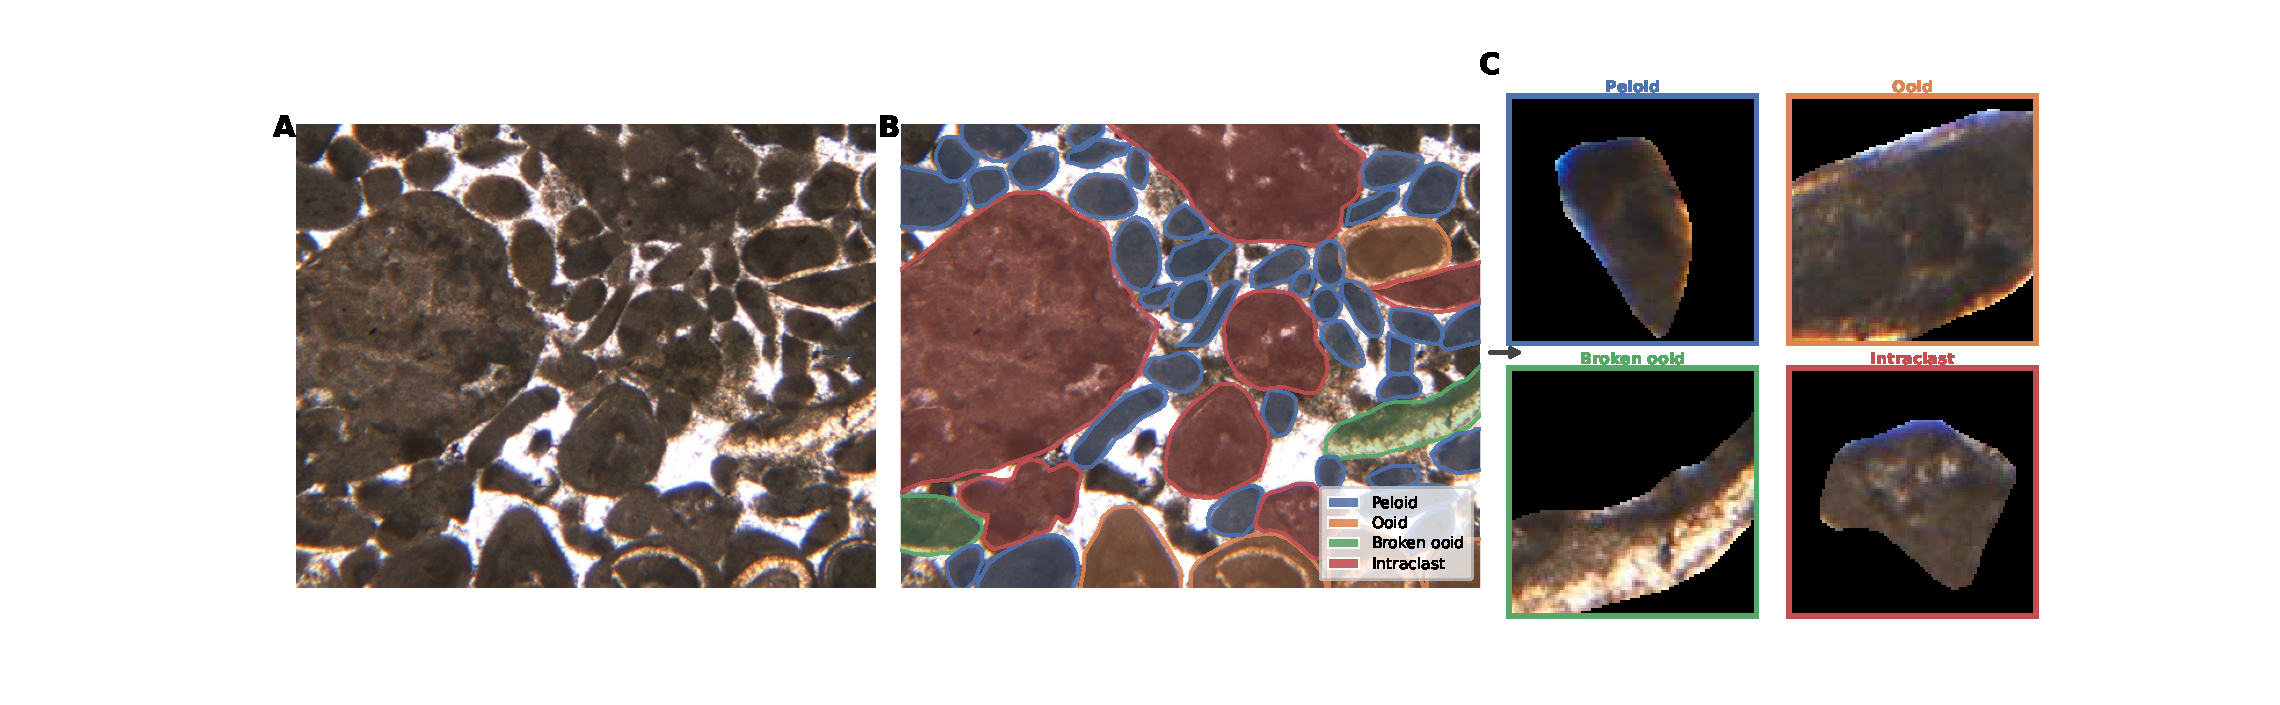
\includegraphics[width=0.97\textwidth]{figs/fig1_pipeline.pdf}
\caption{Data preparation pipeline. \textbf{(A)}~A representative crop from micrograph WT13\_ES0023 in plain polarised light (PPL). \textbf{(B)}~The same crop with LabelMe polygon annotations overlaid; colours identify the four grain classes (blue: Peloid, orange: Ooid, green: Broken ooid, red: Intraclast). \textbf{(C)}~Representative masked 96$\times$96 pixel grain patches extracted from each class; all pixels outside the annotated polygon are set to zero before the patch is passed to the network.}
\label{fig:pipeline}
\end{figure*}

Each grain is represented as a 96$\times$96 pixel RGB patch, cropped from the full thin-section image and centred on the grain's annotated centroid. Before the patch is passed to the network, a binary mask derived from the LabelMe polygon is applied: all pixels outside the grain boundary are set to zero. This ensures that the network sees only the internal morphology and boundary texture of each individual grain, with no contribution from the surrounding cement or matrix. Because every input contains only the pixels interior to a single grain's polygon, two adjacent grains from the same source image share no pixel-level information. Grains from the same micrograph may nonetheless share imaging conditions, preparation artefacts, and local diagenetic context, so annotation-level results should be understood as within-dataset performance rather than a fully independent validation.

The 2,642 grains were divided into training (60\%), validation (20\%), and test (20\%) subsets using stratified random sampling with a fixed random seed of 42, ensuring that class proportions are preserved in each subset. The test set of 529 grains (Peloid: 460, Ooid: 42, Broken ooid: 6, Intraclast: 21) was held out completely during all model development, component selection, and threshold tuning.

Figure~\ref{fig:patches} shows representative grain patches for each class. The visual similarity between peloids and the more diagenetically altered ooid and intraclast examples is apparent even from brief inspection.

\begin{figure*}[t]
\centering
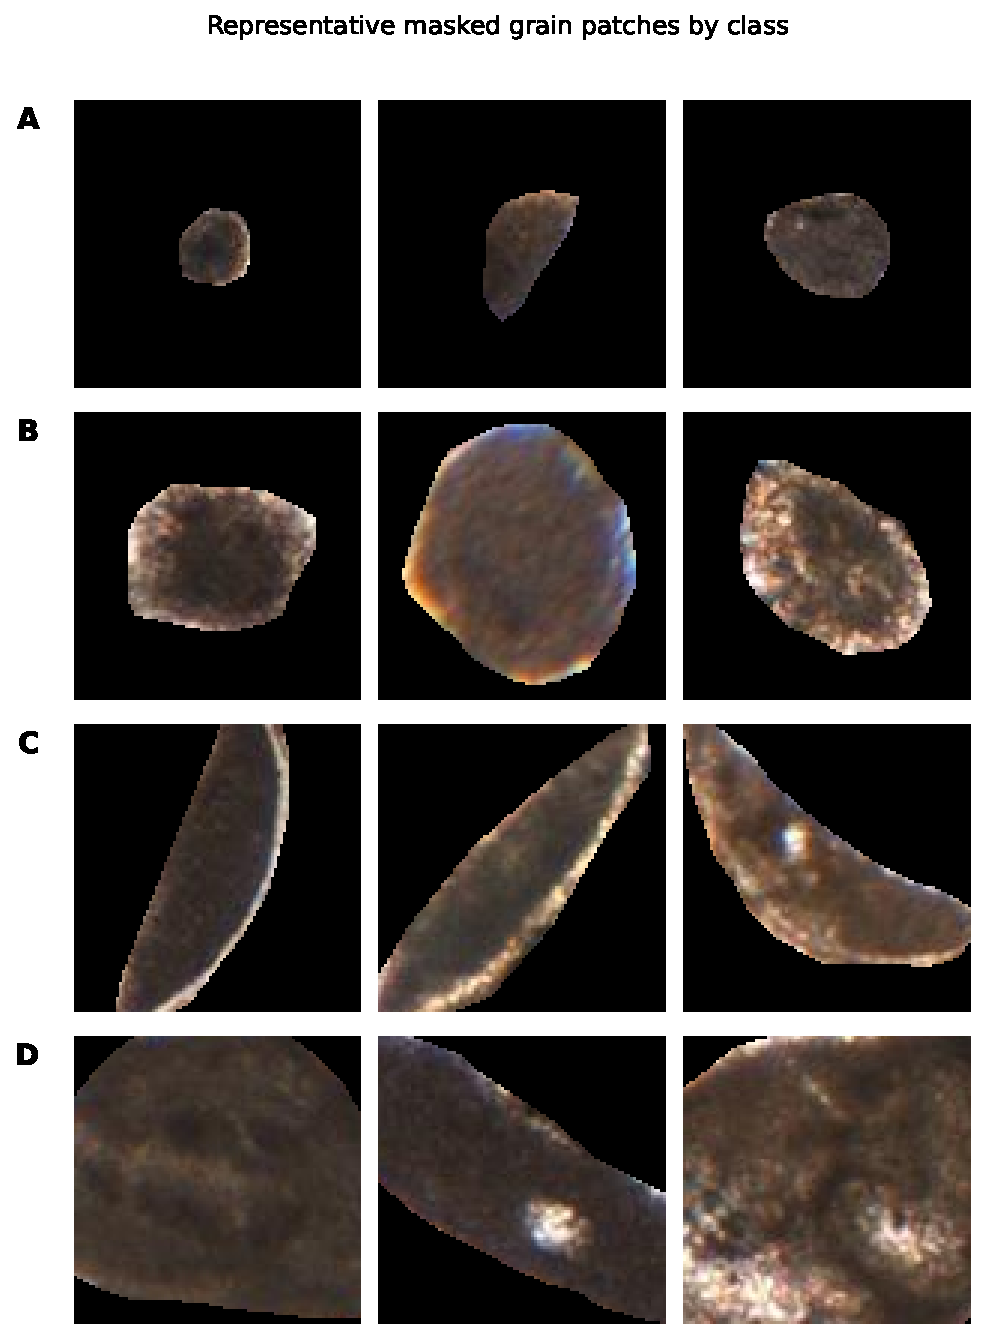
\includegraphics[width=0.85\textwidth]{figs/fig2_sample_patches.pdf}
\caption{Representative 96$\times$96 pixel masked grain patches for each of the four classes (three examples per class): \textbf{(A)}~Peloid, \textbf{(B)}~Ooid, \textbf{(C)}~Broken ooid, \textbf{(D)}~Intraclast. All pixels outside the annotated grain polygon are set to zero. The morphological overlap between peloids and heavily diagenetically altered ooids is visible: both classes show largely structureless, rounded grains with no distinctive internal features. Broken ooids are distinguished by their fractured cortex; intraclasts by remnant angular boundaries or reworked internal fabric.}
\label{fig:patches}
\end{figure*}

\subsection{Model Architecture}

\subsubsection{Hierarchical Decomposition}

A standard deep learning approach maps each input directly to one of four classes via a softmax layer. Under extreme class imbalance, this produces a network whose loss-minimising strategy is to predict peloid for the vast majority of inputs, giving an 87\% overall accuracy that is uninformative for the minority classes.

The approach taken here decomposes the four-class problem into a sequence of binary questions that follow the carbonate grain taxonomy. A grain is first identified as either a peloid or something else. If not a peloid, the question becomes whether it shows the concentric cortical fabric of an ooid-like grain or the angular, reworked texture of an intraclast. If ooid-like, a final question resolves whether the cortex is intact or fractured.

This three-step branching logic is formulated as a sequence of conditional probabilities:
\begin{enumerate}
  \item \textbf{Stage 1:} $P(\text{Peloid} \mid x)$
  \item \textbf{Stage 2:} $P(\text{Ooid-like} \mid x,\ \neg\text{Peloid})$
  \item \textbf{Stage 3:} $P(\text{Broken} \mid x,\ \text{Ooid-like})$
\end{enumerate}

Applying the chain rule, the probability that a grain is an intraclast is:
\begin{equation}
P(\text{Intraclast}) = \bigl(1 - P(\text{Peloid})\bigr) \times \bigl(1 - P(\text{Ooid-like})\bigr)
\end{equation}

This formulation means the Stage 3 head, responsible for the hardest and rarest distinction, never receives gradient updates from the approximately 1,380 peloid training samples.

\subsubsection{Network Structure}

The backbone is ResNet-18 \citep{he2016resnet} initialised with ImageNet pre-trained weights \citep{russakovsky2015imagenet}, which provides a starting point for low-level texture and edge detection without requiring these features to be learned from scratch on a small dataset. The final fully-connected classification layer is removed, leaving a backbone $f_\theta$ that maps each input patch to a 512-dimensional feature vector:
\begin{equation}
h_i = f_\theta(x_i), \quad h_i \in \mathbb{R}^{512}
\end{equation}

This feature vector is passed independently into three binary classification heads, each a compact Multi-Layer Perceptron: Linear(512$\to$128) $\to$ ReLU $\to$ Dropout(0.3) \citep{srivastava2014dropout} $\to$ Linear(128$\to$1). Each head produces a scalar logit, converted to a probability via sigmoid:
\begin{equation}
p_i^{(s)} = \sigma\!\left(MLP^{(s)}(h_i)\right), \quad s \in \{1,2,3\}
\end{equation}

Figure~\ref{fig:architecture} shows the complete architecture.

\begin{figure*}[t]
\centering
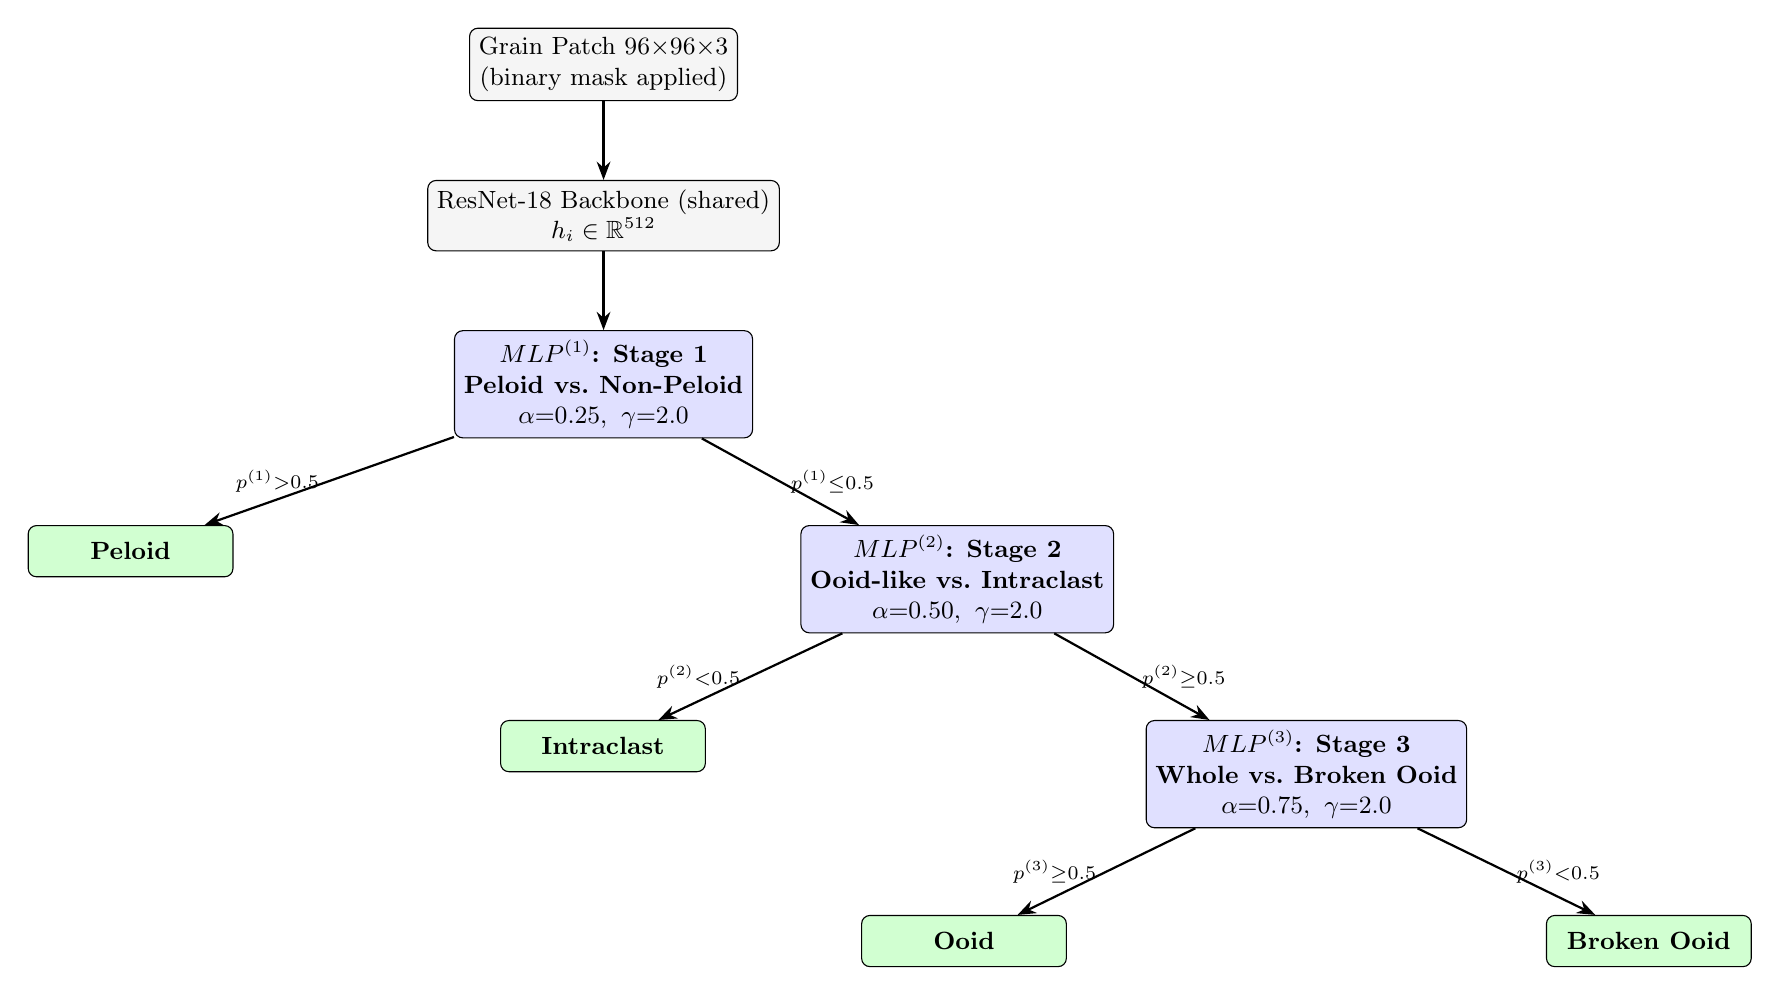
\begin{tikzpicture}[
  node distance=1.0cm and 1.6cm,
  box/.style={draw, rounded corners=3pt, minimum width=3.2cm, minimum height=0.65cm,
              align=center, font=\small, fill=gray!8},
  head/.style={draw, rounded corners=3pt, minimum width=3.6cm, minimum height=0.65cm,
              align=center, font=\small\bfseries, fill=blue!12},
  leaf/.style={draw, rounded corners=3pt, minimum width=2.6cm, minimum height=0.65cm,
              align=center, font=\small\bfseries, fill=green!18},
  arr/.style={-Stealth, thick},
  lbl/.style={font=\scriptsize, midway}
]

\node[box]  (input)    {Grain Patch $96{\times}96{\times}3$\\(binary mask applied)};
\node[box,  below=of input]  (backbone) {ResNet-18 Backbone (shared)\\$h_i \in \mathbb{R}^{512}$};
\node[head, below=of backbone] (mlp1)   {$MLP^{(1)}$: Stage 1\\Peloid vs.\ Non-Peloid\\$\alpha{=}0.25,\ \gamma{=}2.0$};

\node[leaf, below left=1.1cm and 2.8cm of mlp1]  (peloid)    {\textbf{Peloid}};
\node[head, below right=1.1cm and 0.6cm of mlp1] (mlp2)      {$MLP^{(2)}$: Stage 2\\Ooid-like vs.\ Intraclast\\$\alpha{=}0.50,\ \gamma{=}2.0$};

\node[leaf, below left=1.1cm and 1.2cm of mlp2]  (intra)     {\textbf{Intraclast}};
\node[head, below right=1.1cm and 0.4cm of mlp2] (mlp3)      {$MLP^{(3)}$: Stage 3\\Whole vs.\ Broken Ooid\\$\alpha{=}0.75,\ \gamma{=}2.0$};

\node[leaf, below left=1.1cm and 1.0cm of mlp3]  (ooid)      {\textbf{Ooid}};
\node[leaf, below right=1.1cm and 1.0cm of mlp3] (broken)    {\textbf{Broken Ooid}};

\draw[arr] (input)    -- (backbone);
\draw[arr] (backbone) -- (mlp1);
\draw[arr] (mlp1)     -- node[lbl, left]  {$p^{(1)}{>}0.5$}  (peloid);
\draw[arr] (mlp1)     -- node[lbl, right] {$p^{(1)}{\leq}0.5$} (mlp2);
\draw[arr] (mlp2)     -- node[lbl, left]  {$p^{(2)}{<}0.5$}  (intra);
\draw[arr] (mlp2)     -- node[lbl, right] {$p^{(2)}{\geq}0.5$} (mlp3);
\draw[arr] (mlp3)     -- node[lbl, left]  {$p^{(3)}{\geq}0.5$} (ooid);
\draw[arr] (mlp3)     -- node[lbl, right] {$p^{(3)}{<}0.5$}  (broken);

\end{tikzpicture}
\caption{The hierarchical ResNet-18 architecture. A shared backbone extracts a 512-dimensional feature vector from each masked grain patch. Three independent binary classification heads decompose the four-class problem into a sequence of decisions aligned with the geological grain taxonomy. The Focal Loss weighting parameter $\alpha$ is set independently at each head to reflect the local class imbalance at that decision node.}
\label{fig:architecture}
\end{figure*}

\subsection{Training Strategy}

\subsubsection{Stage-Wise Focal Loss}

Under standard binary cross-entropy, gradient contributions are dominated by the majority class even when the network is already confident on those examples. Focal Loss \citep{lin2017focal} addresses this by introducing a modulating factor that down-weights easy, well-classified examples:
\begin{equation}
\mathcal{L}_{FL}(p_t) = -\alpha_t\,(1 - p_t)^{\gamma}\,\log(p_t)
\end{equation}
where $p_t$ is the predicted probability for the correct class, $\gamma$ controls the strength of the down-weighting, and $\alpha_t$ provides explicit per-class balancing.

We set $\gamma = 2.0$ throughout. The key design choice is that $\alpha$ is not shared across heads but calibrated separately based on the local imbalance at each binary decision:
\begin{itemize}
  \item \textbf{Stage 1} (Peloid vs.\ Non-Peloid): $\alpha = 0.25$. This head faces the most extreme imbalance (87\% peloid), so the minority class receives a strong weighting correction.
  \item \textbf{Stage 2} (Ooid-like vs.\ Intraclast): $\alpha = 0.50$. Within the non-peloid sub-population, the imbalance is less severe, so a symmetric weighting is appropriate.
  \item \textbf{Stage 3} (Whole Ooid vs.\ Broken Ooid): $\alpha = 0.75$. Broken ooids are the minority within ooid-like grains, so the weighting shifts modestly toward them.
\end{itemize}

\subsubsection{Targeted Oversampling}
\label{sec:oversampling}

Even with Focal Loss, having fewer than 20 training examples of a class means gradient updates from that class are sparse. Broken ooid grains are therefore oversampled at 15 times their natural frequency: each broken ooid in the training set appears 15 times per epoch, while batch composition is arranged so that each mini-batch contains 50\% peloid and 50\% non-peloid samples.

The oversampling uses real grain patches repeated with standard training augmentations (random 90° rotation, horizontal and vertical flip, modest brightness and contrast adjustment). This differs from synthetic augmentation methods such as SMOTE \citep{chawla2002smote}: the network sees the same grains from slightly different perspectives, not interpolated synthetic grains.

\subsubsection{Four-Phase Staged Training Curriculum}
\label{sec:staged_training}

A failure mode in multi-head architectures trained on imbalanced data is backbone monopolisation. Because Stage 1 is both the most gradient-heavy decision and the most easily solved, it tends to steer the shared backbone's weights toward peloid-relevant features during joint training. When Stage 2 and Stage 3 heads then receive features from a backbone oriented primarily toward peloid detection, they are working with representations less suited to fine-grained distinctions.

Training proceeds in four sequential phases to address this:

\begin{enumerate}
  \item \textbf{Phase 1: Head initialisation} (10 epochs, lr $= 1\times10^{-3}$): The backbone is frozen with its ImageNet weights. All three heads are trained simultaneously. This establishes reasonable head weights before any backbone adaptation.

  \item \textbf{Phase 2: Backbone tuning for Stage 1} (15 epochs, lr $= 1\times10^{-4}$): The backbone is unfrozen. Only the Stage 1 head receives gradient updates; Stages 2 and 3 are frozen. The backbone adapts specifically for peloid detection.

  \item \textbf{Phase 3: Minority-class head optimisation} (15 epochs, lr $= 1\times10^{-4}$): Stage 1 is frozen. Stages 2 and 3 are trained on oversampled batches. With a backbone already adapted for the peloid/non-peloid distinction, the minority-class heads have access to more useful feature representations.

  \item \textbf{Phase 4: Full fine-tuning} (10 epochs, lr $= 1\times10^{-5}$): All parameters are unfrozen and trained jointly at a low learning rate, allowing the network to settle without disrupting Phase 3 gains.
\end{enumerate}

The best checkpoint across all 50 epochs is selected based on validation Balanced Accuracy. Figure~\ref{fig:training_curve} shows how validation Balanced Accuracy evolves across the four phases.

\subsubsection{Inference-Time Augmentation}
\label{sec:tta}

Grains near a decision boundary can produce unstable predictions from a single deterministic forward pass \citep{shanmugam2021tta}. Each grain is therefore passed through the network six times, under six geometric transformations that preserve grain morphology: the original orientation, horizontal flip, vertical flip, and rotations by 90°, 180°, and 270°. The six sets of logits are averaged before the final decision:
\begin{equation}
\hat{p}_i = \frac{1}{6}\sum_{k=1}^{6} p\!\left(y \mid T_k(x_i),\, \theta\right)
\end{equation}

Averaging over orientations is appropriate for grain images because real grains are deposited with arbitrary rotational orientation and there is no natural upright direction.

\subsubsection{Implementation Details}

All models were implemented in PyTorch \citep{paszke2019pytorch}. Training was performed on a Google Colab environment using an NVIDIA GPU. The AdamW optimiser \citep{loshchilov2019adamw} was used with a weight decay of $1\times10^{-4}$. Each classification head comprises two linear layers (512$\to$128 and 128$\to$1) with biases, totalling 65,793 parameters per head, small relative to the 11.2 million parameters in the shared backbone.

\subsubsection{Evaluation Metrics}

Overall accuracy is misleading at this level of class imbalance: a model predicting peloid for every grain achieves 87\% without learning anything useful. Balanced Accuracy \citep{brodersen2010balanced}, the arithmetic mean of per-class recall, is therefore used as the primary metric:
\begin{equation}
\text{Balanced Accuracy} = \frac{1}{4}\sum_{c=1}^{4} \frac{TP_c}{TP_c + FN_c}
\end{equation}

This gives equal weight to correctly identifying a broken ooid (6 test samples) and a peloid (460 test samples), which matches the scientific objective. Overall Accuracy is also reported for completeness. For class-level estimates based on very small sample counts, particularly the 6 broken ooid test instances, the 95\% Wilson confidence interval is wide: a recall of 5/6 spans [36\%--97\%]. Comparisons between models on this class alone are not statistically reliable.

%%=============================================================
\section{Results}
%%=============================================================

\subsection{Baseline Comparisons}

Two baselines are reported for context. The flat ResNet-18 was evaluated on the same held-out test set as the hierarchical model; the SAM+XGBoost pilot used a separate image-level hold-out split and is not directly comparable.

The first is the SAM-based pilot described in the Introduction: the Segment Anything Model \citep{kirillov2023sam} applied for zero-shot grain segmentation, followed by XGBoost \citep{chen2016xgboost} trained on 65 hand-crafted geometric, textural, and colorimetric features extracted from the resulting masks. Evaluated on a separate image-level hold-out split, it achieves 80.9\% Balanced Accuracy, with ooid precision 48.7\% and intraclast precision 24.7\%. Because this evaluation used a different data partition from the annotation-level split used for all deep learning experiments, per-class recall figures are not directly comparable and are omitted from Table~\ref{tab:ablation}; the 80.9\% figure is reported here for context only.

The second baseline is a flat ResNet-18 with a four-class softmax output trained with standard cross-entropy loss, without hierarchical structure, oversampling, or Focal Loss. On the test set it achieves 86.9\% Balanced Accuracy and 95.5\% Overall Accuracy, with per-class recall of 97.6\% for peloids, 88.1\% for ooids, 100\% (6/6) for broken ooids, and 61.9\% for intraclasts. The 100\% broken ooid recall deserves careful interpretation: with six test instances, one prediction separates 83.3\% recall from 100\%, and the 95\% Wilson confidence interval for 6/6 spans [54\%--100\%]. This result does not indicate that the flat model has reliably learned to detect broken ooids; it reflects statistical noise inherent in evaluating a class with six samples. The flat model's intraclast recall of 61.9\% is substantially below what the hierarchical approach achieves.

\subsection{Component Ablation}
\label{sec:results_ablation}

Table~\ref{tab:ablation} shows per-class recall as each pipeline component is added to the hierarchical base architecture.

\begin{table*}[t]
\centering
\caption{Per-class recall on the 529-grain held-out test set as pipeline components are added sequentially. Balanced Accuracy (BA) is the arithmetic mean of the four per-class recall values. Overall Accuracy (OA) is included for reference. Bold entries indicate the best result among hierarchical configurations in each column. $^\dag$The flat baseline's 100\% broken ooid recall rests on 6 out of 6 test instances; the 95\% Wilson confidence interval is [54\%--100\%].}
\label{tab:ablation}
\resizebox{\textwidth}{!}{%
\begin{tabular}{lcccccc}
\toprule
\textbf{Model} & \textbf{Peloid (N=460)} & \textbf{Ooid (N=42)} & \textbf{Broken ooid (N=6)} & \textbf{Intraclast (N=21)} & \textbf{BA} & \textbf{OA} \\
\midrule
Flat ResNet-18, cross-entropy (baseline)$^\dag$ & 449 (97.6\%) & 37 (88.1\%) & 6 (100\%)  & 13 (61.9\%)  & 86.9\%       & 95.5\% \\
Hierarchical ResNet-18, no oversampling         & 442 (96.1\%) & 33 (78.6\%) & 1 (16.7\%) & 13 (61.9\%)  & 63.3\%       & 92.4\% \\
+ 15$\times$ oversampling                        & \textbf{454 (98.7\%)} & 35 (83.3\%) & 4 (66.7\%) & 13 (61.9\%) & 77.7\%       & 95.7\% \\
+ 15$\times$ oversampling + TTA                  & \textbf{454 (98.7\%)} & \textbf{37 (88.1\%)} & 4 (66.7\%) & 14 (66.7\%) & 80.0\%       & \textbf{96.2\%} \\
+ Staged training + oversampling + TTA \textbf{(full model)} & 431 (93.7\%) & 36 (85.7\%) & \textbf{5 (83.3\%)} & \textbf{15 (71.4\%)} & \textbf{83.5\%}  & 92.1\% \\
\bottomrule
\end{tabular}%
}
\end{table*}

The hierarchical network without oversampling recovers only 16.7\% of broken ooid instances (one grain out of six), despite having the same branching structure, stage-wise Focal Loss, and pre-trained backbone as the full model. Adding 15$\times$ targeted oversampling raises broken ooid recall to 66.7\% in a single step and lifts Balanced Accuracy from 63.3\% to 77.7\%.

Adding inference-time augmentation on top of oversampling improves ooid recall from 83.3\% to 88.1\% and intraclast recall from 61.9\% to 66.7\%, raising Balanced Accuracy to 80.0\%. The full model, which adds the four-phase staged training curriculum, achieves 83.5\% Balanced Accuracy. Peloid recall drops from 98.7\% to 93.7\% relative to the oversampling-only configuration, while broken ooid recall rises from 66.7\% to 83.3\% and intraclast recall from 66.7\% to 71.4\%.

\subsection{Confusion Matrix and Precision-Recall Curves}

Table~\ref{tab:confusion} shows the confusion matrix for the full model. Figure~\ref{fig:pr_curves} shows per-class Precision-Recall curves evaluated on the test set using continuous probability scores.

\begin{table}[h]
\centering
\caption{Confusion matrix for the full model: hierarchical ResNet-18 with four-phase staged training, 15$\times$ oversampling, and inference-time augmentation. Rows are true classes; columns are predicted classes.}
\label{tab:confusion}
\begin{tabular*}{\tblwidth}{@{}lcccc@{}}
\toprule
\textbf{Actual $\backslash$ Predicted} & \textbf{Peloid} & \textbf{Ooid} & \textbf{Broken ooid} & \textbf{Intraclast} \\
\midrule
\textbf{Peloid}       & 431 & 11 & 0 & 18 \\
\textbf{Ooid}         &   3 & 36 & 3 &  0 \\
\textbf{Broken ooid}  &   0 &  0 & 5 &  1 \\
\textbf{Intraclast}   &   3 &  2 & 1 & 15 \\
\bottomrule
\end{tabular*}
\end{table}

\begin{figure*}[t]
\centering
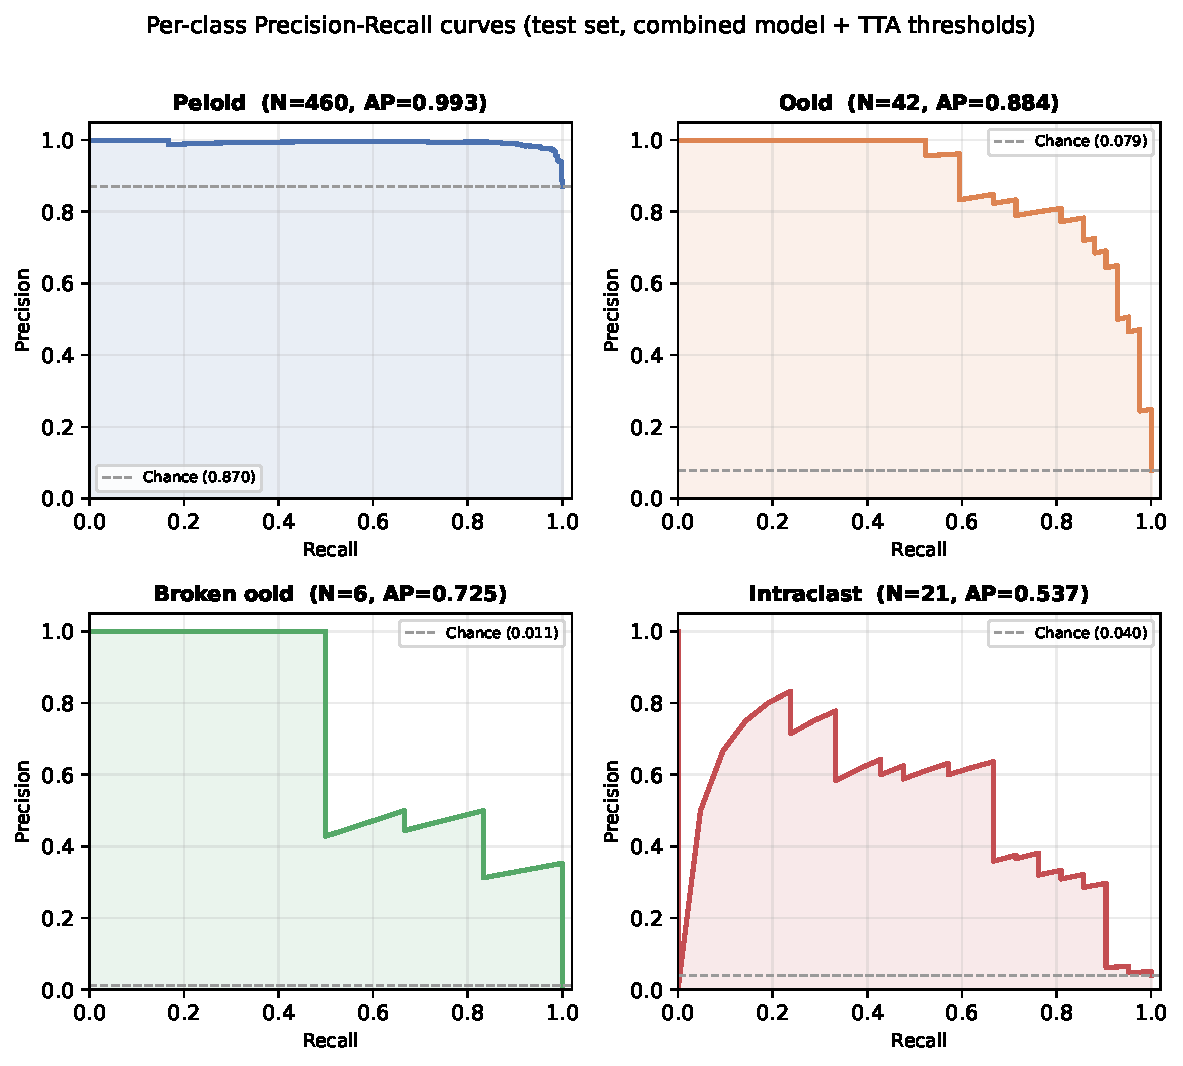
\includegraphics[width=0.92\textwidth]{figs/fig4_pr_curves.pdf}
\caption{Per-class Precision-Recall curves for the full model on the 529-grain test set. Each subplot shows the curve for one class against the random-classifier baseline (dashed line, equal to class prevalence in the test set). AP denotes Average Precision (area under the curve). The narrow curves for broken ooid and intraclast reflect the small number of positive test instances for those classes.}
\label{fig:pr_curves}
\end{figure*}

%%=============================================================
\section{Discussion}
%%=============================================================

\subsection{The Role of Each Pipeline Component}

The ablation results establish a clear ordering of importance among the pipeline components.

Oversampling has the largest single effect of any component. Without it, the hierarchical base model recovers only 16.7\% of broken ooids despite having the branching architecture, stage-wise Focal Loss, and pre-trained backbone of the full model. Architecture alone cannot compensate for the near-absence of broken ooid gradient signal when fewer than 20 training examples are available. The 15$\times$ oversampling factor provides the Stage 3 head with sufficient training signal to learn a decision boundary.

Inference-time augmentation contributes independently of oversampling, primarily by stabilising predictions for grains near decision boundaries. The most consistent beneficiary is the ooid class, where recall improves by 4--5 percentage points. This is consistent with the rotationally symmetric nature of the ooid cortex: a network that learned orientation-specific edge patterns during training classifies the same grain more confidently once those orientations are averaged.

The staged training curriculum produces the most nuanced effect. It does not dramatically change any single class's recall but achieves the most consistently balanced distribution across all four classes simultaneously. By directing the backbone's gradient updates toward the fine-grained distinctions between ooid-like grains and intraclasts during Phase 3, the curriculum improves intraclast recall from 66.7\% to 71.4\% while simultaneously raising broken ooid recall from 66.7\% to 83.3\%. The cost is a reduction in peloid recall from 98.7\% to 93.7\%.

\subsection{Comparison with the Flat Baseline}

The flat ResNet-18 achieves a higher headline Balanced Accuracy (86.9\%) than the full hierarchical model (83.5\%) on this test split, and a higher Overall Accuracy (95.5\% vs.\ 92.1\%). This difference is driven entirely by broken ooid recall: the flat model correctly classifies all six broken ooid test instances, while the hierarchical model classifies five. As noted above, the 95\% Wilson confidence interval for a 6/6 result spans [54\%--100\%]; a single different outcome would reverse the ranking. The hierarchical model's advantage in intraclast recall (71.4\% vs.\ 61.9\%), based on 21 test instances, is more statistically stable.

The flat model's performance on this particular test split does not indicate that it has learned a stable representation of broken ooids. With six test instances, one prediction separates 83.3\% from 100\%; the result is split-dependent. The structural argument for the hierarchical design is gradient isolation: in a flat four-class model, the gradient from approximately 1,380 peloid training examples flows equally to all output neurons, including the broken ooid neuron. In the hierarchical model, the Stage 3 head, responsible for the intact versus broken decision, receives gradient only from ooid-like grains, approximately 143 training examples (126 intact ooid and 17 broken ooid instances in the training split), never from peloids. Oversampling broken ooids within that sub-population is more effective than oversampling them within the full peloid-dominated training set, because the backbone is not simultaneously being pulled toward peloid-relevant features. We report both results because honest evaluation, including cases where a simpler baseline is not clearly dominated on headline metrics, is necessary for the field to progress.

\subsection{Latent Space Structure}

Figure~\ref{fig:tsne} shows a two-dimensional t-SNE \citep{vandermaaten2008tsne} projection of the 512-dimensional backbone feature vectors for all 529 test-set grains. The clearest feature is the separation between the peloid cluster and the non-peloid classes, consistent with Stage 1 learning a reliable boundary during Phase 2 of the staged curriculum. Ooids, broken ooids, and intraclasts occupy an overlapping region, reflecting their genuine morphological similarity and explaining why Stages 2 and 3 are harder problems than Stage 1.

\begin{figure*}[t]
\centering
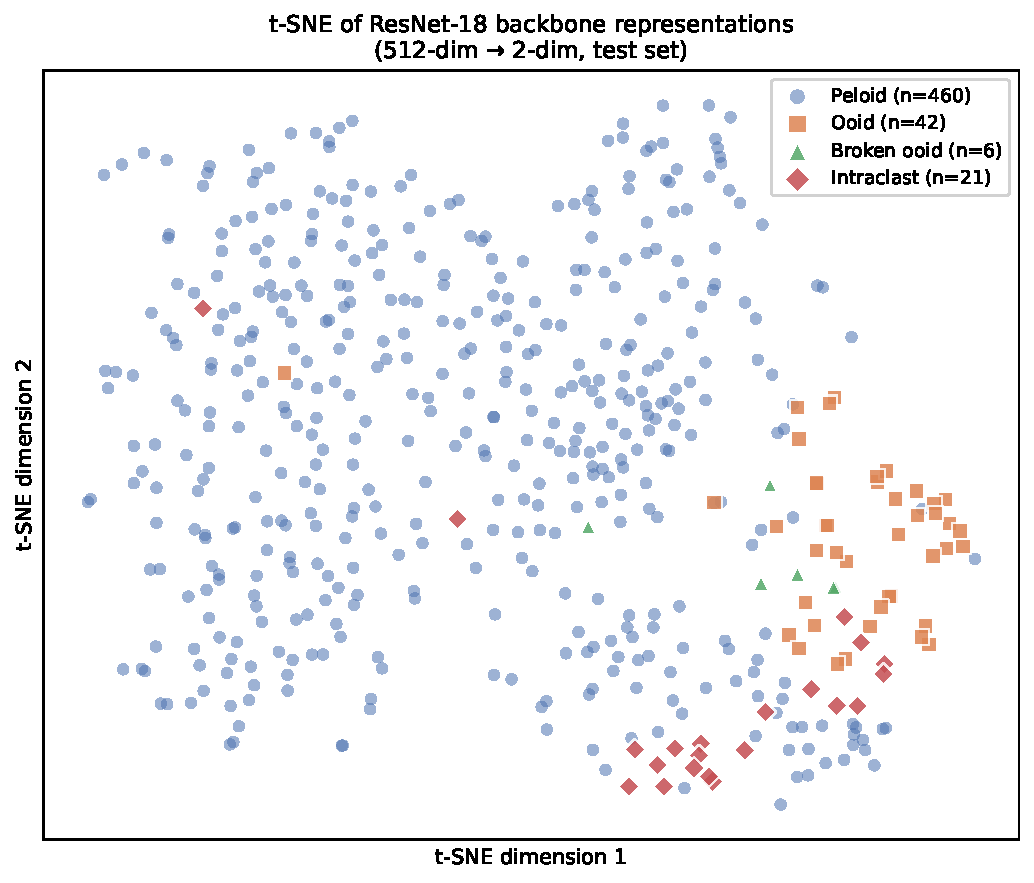
\includegraphics[width=0.75\textwidth]{figs/fig5_tsne.pdf}
\caption{Two-dimensional t-SNE projection of the 512-dimensional ResNet-18 backbone features for all 529 test-set grains, coloured by true class. Peloids form a broad, dense cluster separated from the non-peloid classes, consistent with the Stage 1 decision boundary. Ooids, broken ooids, and intraclasts occupy an overlapping region.}
\label{fig:tsne}
\end{figure*}

\begin{figure*}[t]
\centering
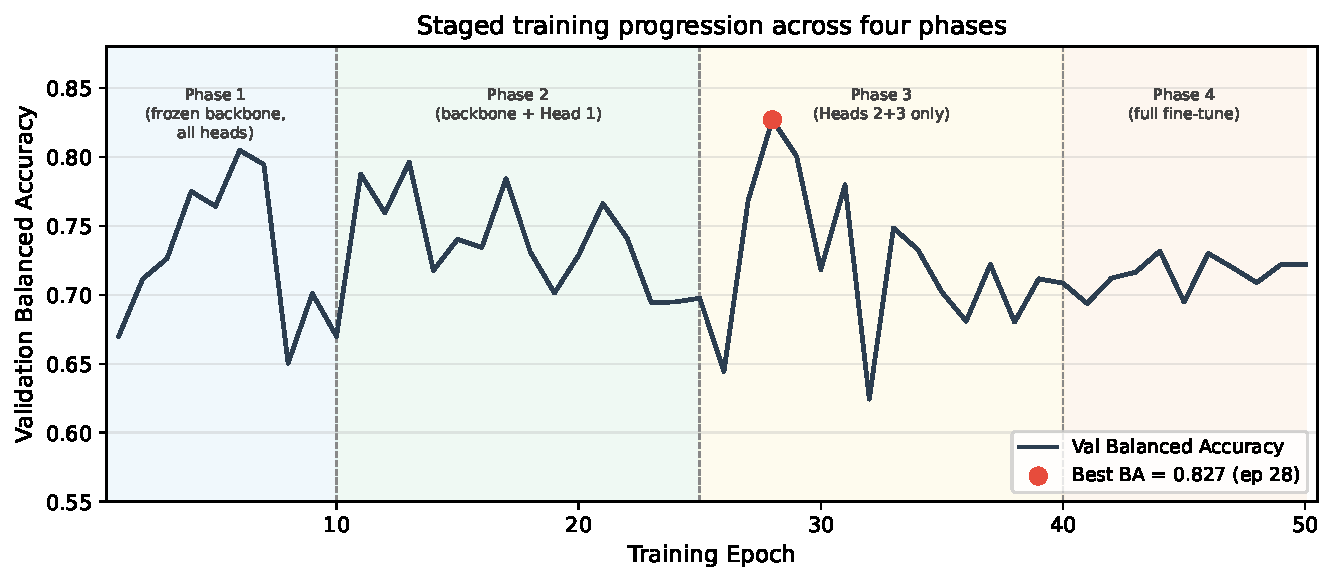
\includegraphics[width=0.92\textwidth]{figs/fig3_training_curve.pdf}
\caption{Validation Balanced Accuracy across all 50 training epochs, with vertical dashed lines separating the four training phases. The best checkpoint is selected at the peak Balanced Accuracy within Phase 3, at which point minority-class head optimisation on an already-adapted backbone produces the best overall class balance.}
\label{fig:training_curve}
\end{figure*}

\subsection{The Peloid--Intraclast Confusion and Its Geological Interpretation}

% NOTE FOR mr. GALLOIS: Please review and expand this subsection.
% Key questions: (1) Do the Peloid-Intraclast confusions correspond to
% specific diagenetic facies in this material? (2) Can you confirm the
% depositional significance of Broken Ooid occurrences in this succession?

The dominant error in the confusion matrix (18 peloids classified as intraclast, and 3 intraclasts classified as peloid) reflects an ambiguity familiar to carbonate sedimentologists. Figure~\ref{fig:misclassifications} shows representative examples of both error directions from the test set.

Peloids and intraclasts can be morphologically indistinguishable when diagenesis is advanced. Both may present as sub-rounded grains with structureless micrite interiors. The defining criterion for an intraclast, the presence of remnant sedimentary fabric or angular reworked edges, becomes increasingly difficult to detect as micritisation progresses \citep{flugel2010}. Human analysts working with comparable material encounter the same boundary, and many published petrographic descriptions acknowledge it explicitly as a zone of interpretive uncertainty.

The direction of the model's errors is also consistent with the training design: the 15$\times$ oversampling and the Stage 2 head's $\alpha = 0.50$ Focal Loss weighting create a training environment biased toward detecting non-peloid features. A peloid with unusually irregular or angular boundaries occupies an ambiguous position in the classification space and is more likely to be captured by the intraclast detector than to pass through as a peloid.

Five of the six broken ooid test instances were correctly identified. Broken ooids are produced by mechanical fracture of intact ooid cortices during high-energy agitation: storm events, strong tidal currents, or wave-driven reworking. Their presence in a thin section is a direct indicator of a high-energy depositional environment, and their abundance relative to intact ooids can constrain the intensity and duration of such events within a carbonate succession.

\begin{figure}[t]
  \centering
  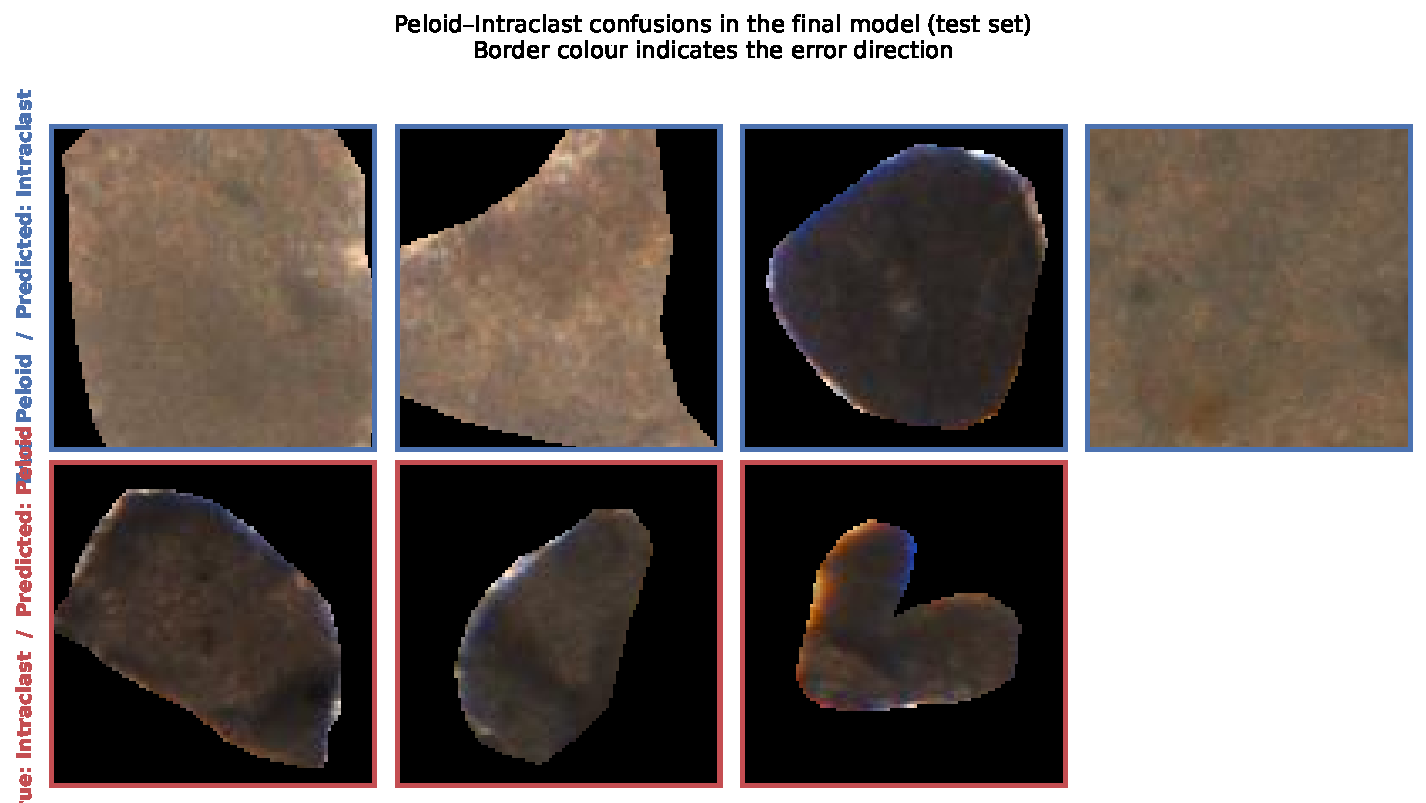
\includegraphics[width=\linewidth]{figs/fig6_misclassifications.pdf}
  \caption{Representative misclassified grains from the test set illustrating the Peloid--Intraclast boundary. \textit{Top row}: peloid grains predicted as intraclasts. \textit{Bottom row}: intraclast grains predicted as peloids. In each case, advanced micritisation has obscured the textural features that would allow confident assignment to one class.}
  \label{fig:misclassifications}
\end{figure}

\subsection{Comparison with Published Methods}

Table~\ref{tab:comparison} places these results alongside closely related published methods. Direct numerical comparison is not meaningful because datasets, class counts, and evaluation protocols differ across studies; the table contextualises the difficulty of the task.

\begin{table*}[t]
\centering
\caption{Contextual comparison with published methods on related petrographic classification tasks. This study operates under the most severe class imbalance of the listed studies ($\sim$79:1 peloid-to-broken-ooid ratio). Balanced Accuracy and Overall Accuracy are reported; other studies report Overall Accuracy only.}
\label{tab:comparison}
\resizebox{\textwidth}{!}{%
\begin{tabular}{llllcc}
\toprule
\textbf{Study} & \textbf{Method} & \textbf{Task} & \textbf{Classes} & \textbf{Metric} & \textbf{Result} \\
\midrule
\citet{pireslima2020}   & Fine-tuned CNN                     & Microfacies, Sycamore Fm.       & 5  & OA  & 90\% (in-domain) / 40\% (cross-domain) \\
\citet{liu2020}         & Inception ResNet v2                & Fossils \& abiotic, 30k images  & 22 & OA  & 95\% \\
\citet{ho2023}          & TaxonNet (hierarchical CNN)        & Carbonate skeletal grains       & 3  & OA  & $\sim$95\% \\
\citet{liudunham2023}   & DenseNet121 + VGG + U-Net          & Dunham textures, Hanifa Fm.     & 5  & OA  & 89\% \\
\textbf{This study}     & \textbf{Hierarchical ResNet-18 + staged training + TTA} & \textbf{Carbonate grain types, $\sim$79:1 imbalance} & \textbf{4} & \textbf{BA / OA} & \textbf{83.5\% / 92.1\%} \\
\bottomrule
\end{tabular}%
}
\end{table*}

The accuracy figures from \citet{pireslima2020}, \citet{ho2023}, and \citet{liudunham2023} are all Overall Accuracy, not Balanced Accuracy; applying Balanced Accuracy to their results would likely yield lower numbers given the unequal class distributions in those studies. The cross-domain collapse reported by \citet{pireslima2020} (90\% in-domain accuracy falling to 40\% on samples from a different laboratory) illustrates the brittleness of flat architectures under distribution shift. The TaxonNet result \citep{ho2023} is architecturally similar but operates on taxonomically distinct grain groups with substantially lower inter-class morphological overlap.

\subsection{Limitations}

\textbf{Dataset size and scope.} The dataset comprises 2,642 grains from 18 micrographs of a single carbonate succession. The model has encountered only a limited range of diagenetic textures, preparation artefacts, and imaging conditions. Whether the learned representations transfer to carbonates from different formations, laboratory preparations, or imaging systems remains untested. \citet{dawson2023dataset} showed that CNNs trained on small carbonate datasets overfit even with transfer learning, and the cross-laboratory collapse documented by \citet{pireslima2020} confirms this is a genuine risk.

\textbf{Statistical uncertainty on broken ooids.} There are only six broken ooid instances in the test set. A single misclassification shifts the per-class recall estimate by 16.7 percentage points, and the 95\% Wilson confidence interval for the observed 83.3\% recall (5/6) spans from 36\% to 97\%. Any claim about broken ooid detection performance based on this test set alone is indicative rather than definitive.

\textbf{Peloid recall trade-off.} The staged training curriculum improves Balanced Accuracy at the cost of peloid recall, which drops from 98.7\% to 93.7\%. For applications where peloid identification is as important as minority-class detection, this trade-off may need to be reconsidered.

\textbf{Backbone architecture.} ResNet-18 was chosen for computational efficiency and established suitability for fine-tuning on small datasets. More expressive backbones (Vision Transformers, EfficientNet, or larger ResNet variants) might extract more discriminative features, but would require substantially more annotated data to avoid overfitting under these class imbalance conditions.

%%=============================================================
\section{Conclusion}
%%=============================================================

Carbonate microfacies classification is a difficult machine learning problem not because the images are inherently complex, but because the class distribution is extreme and the minority classes are defined by subtle morphological signals that standard training procedures fail to recover. This paper has described a concrete path through that difficulty: encode the geological taxonomy of carbonate grains directly into the network's branching structure, calibrate the loss function separately at each decision node to reflect the local class imbalance, oversample the most underrepresented class at the batch level, train in a staged sequence that prevents the majority-class head from monopolising the shared backbone, and average predictions over multiple orientations at inference time to stabilise boundary decisions.

Oversampling has the largest single effect on minority-class detection. The hierarchical base without it achieves only 16.7\% recall for broken ooids. Oversampling raises this to 66.7\% and Balanced Accuracy to 77.7\%; adding inference-time augmentation raises Balanced Accuracy to 80.0\%. The staged training curriculum produces a more distributed improvement: no single class gains dramatically, but all four classes are better balanced simultaneously, with no class falling below 71\% recall in the full model.

On the held-out test set of 529 grains, the complete pipeline achieves 83.5\% Balanced Accuracy and 92.1\% Overall Accuracy. Five of the six broken ooid instances are correctly identified, a class that the unmodified hierarchical base nearly misses entirely. The primary remaining error is Peloid--Intraclast confusion, which reflects a genuine geological ambiguity that human analysts also find difficult in heavily diagenetically altered material.

Several directions remain open for future work. The most immediate need is evaluation on independent carbonate successions to test whether the learned representations generalise across geological settings and laboratory preparations. Sedimentology-driven synthetic data generation approaches such as SynSection \citep{ransinangue2025synsection} offer a path toward augmenting scarce minority-class training data without departing from geologically valid grain morphologies. Within the current framework, investigating class-specific inference strategies, for example applying orientation averaging only to the ooid-related decisions while using deterministic inference for intraclasts (which are partly defined by their asymmetric shape), may recover some of the intraclast recall that the current global averaging approach sacrifices.

\printcredits

\bibliographystyle{cas-model2-names}
\bibliography{references}

\bio{}
Musawer Muradi is a researcher in the Department of Computer Engineering at Kocaeli University. His research interests include deep learning, computer vision, and the application of machine learning to geological data analysis.
\endbio

\bio{}
Arnaud Gallois is a geologist in the Department of Geological Engineering at Kocaeli University, specialising in carbonate sedimentology and petrographic analysis of lacustrine and shallow-marine carbonate successions.
\endbio

\bio{}
Alev Mutlu is a faculty member in the Department of Computer Engineering at Kocaeli University with research interests in data science and computational methods for earth sciences.
\endbio

\end{document}
